\section{Project Stage}
\subsection{System Architecture}

\begin{figure}[H]
	\centering
	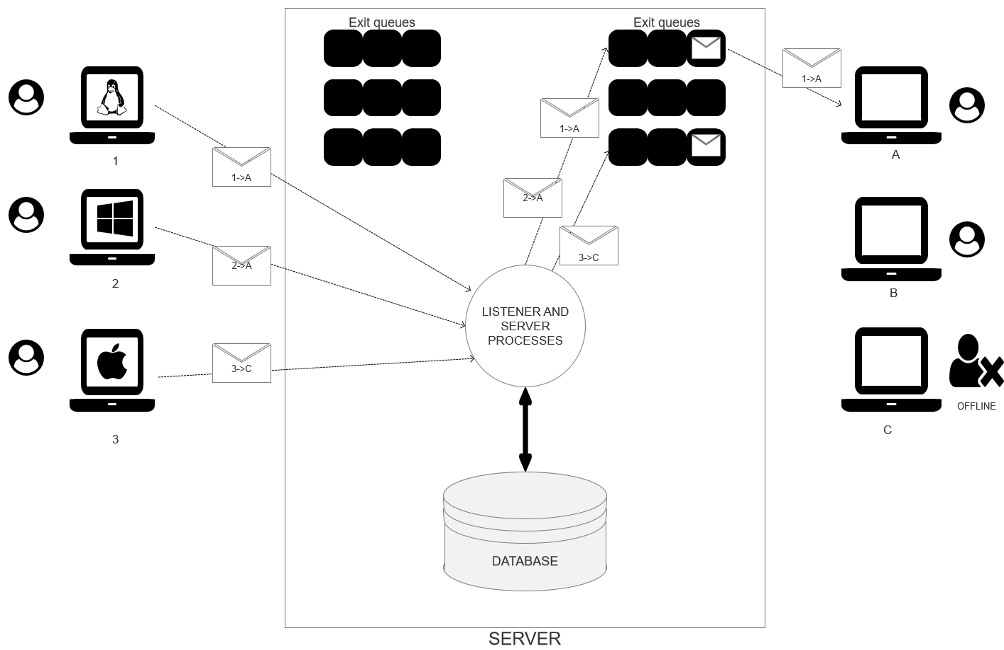
\includegraphics[width=\textwidth]{img/systemArchitecture.png}  
\end{figure}

As shown in the previous picture, the application is based on a client-server architecture, in which each client, in order to send a \textbf{message} to a \textbf{user}, contacts the main server which is in charge of determining receiver’s physical address and forward the \textbf{message} if it is online.
In the image some typical scenarios are represented to help better understand how \textit{Unisup} works. In particular:
\begin{enumerate}
	\item The message 1 $\xrightarrow{}$ A is sent from the client 1 destined to the client A:  it arrives at the main server that pushes it into the corresponding queue. The client A is online and there is no message to consume on the queue, so it is immediately forwarded.
	\item The message 2 $\xrightarrow{}$ A is sent from the client 2 destined to the client A:  as the previous one, it is pushed into A’s queue but this time the channel is busy. The message will be forwarded as soon as the channel comes idle again.
	\item The message 3 $\xrightarrow{}$ C is sent from client 3 destined to C: again, it is pushed on the correct queue. C is offline, so the message is not forwarded; it will be delivered as soon as C turns online again.
\end{enumerate}	
The OS picture inside clients means that the system works on every OS.
Eventually, the database icon has been added since it is required for mapping clients’ addresses and store chat histories. 


\subsection{Clients}
\subsubsection{Role of the Client}
During the normal usage of the application, the users interact with their client device, so the client is the principal actor of our application.
As described in the use cases analysis user i can register to the application, sign in into his/her account, then he/she can do all the operation of a typical instant-message application like sending/receiving messages and read old messages through clicking on chats. Because the applicative isn’t bound to a specific client, as \textit{Whatsapp} is, a client device can be used by multiple \textbf{users}, they only need to register/login to their account.
From an architectural point of view, the \textbf{client} is only in charge of providing the \textbf{user} a GUI and the communication with the server. The \textbf{client}  device does not store the history of the messages, nor information about the user, but it is in charge of showing chats and messages in the correct natural order that is sorted by ascending timestamp. On client-side, a multithreaded approach has been developed according to the following DAG.

Since SEND A MESSAGE and RECEIVE A MESSAGE are concurrent actions, they are performed by different flows of execution. The only shared data structured is the message list of the relative chat, so the access to it must be synchronized.

\subsubsection{Technologies}
The applicative code runs entirely on the clients: every interaction with the GUI is handled locally and may trigger a send request to the server. The principles technologies used in the client side are JavaFX and Jinterface.
\begin{itemize}
	\item The GUI is implemented using JavaFX classes, some of them were extended for creating ad-hoc classes that can be found in the javafxexstension package. The use of JavaFX is due to make the application more user-friendly.
	\item The Jinterface package provides a set of tools for communication with Erlang processes. In this way the client can send and receive messages to the server, define receive mailboxes and so on.
\end{itemize}

\subsection{The Server}
\subsubsection{Role of the Server}
The server is the core of our system, every client has to communicate with it in order to accomplish any operation of that one’s listed in chapter 2.1.
The server is in charge of:

\begin{itemize}
	\item Register user data at registration time, remembering username and password.
	\item Login users by checking username and password, binding usernames with the physical client process in charge of the receiving of the message.
	\item Forward any message to the correct client: every sender client contacts firstly the server (so that clients are not requested to store physical addresses of other clients, they specify WHAT and not HOW to deliver messages). The server is capable, having as input a username, of determining the relative physical address and forward the message.
	\item Register every in-transit message in order to permit the restoring of the chat list for every client
	\item Queuing correctly the messages that are destined to the same client, so that to handle concurrency and buffering of messages whose receiver is offline. 
\end{itemize}

\subsubsection{Implementation of the Server}
In order to achieve a high-performance application, it is crucial to have a lightweight \textbf{server} code, capable of handling quickly every request and of parallelizing work when possible. As discussed in the paragraph 3.2.1, concurrent actions inside a \textbf{client} are handled by the \textbf{client} itself; the \textbf{server}  is in charge of handling concurrency between different \textbf{clients}. In order to accomplish these requirements, we chose to implement the server entirely in Erlang, so that:
\begin{itemize}
	\item The lightweight of the language is particularly suitable to ensure high performance on the simple actions that the server must perform
	\item The Mnesia persistent support guarantees fast operations and internal handling of concurrent accesses to the data (see par. 3.3.3)
	\item The RabbitMq library queues messages destined to every client with a FIFO policy. It ensures correct concurrency handling and buffering of messages whose receiver is offline.
\end{itemize}
In addition, to improve performance and abstract the \textbf{server} structure, we decided to adopt the \textit{Gen\_Server} behavior to handle \textbf{client} requests.
Moreover, to decrease the coupling between \textbf{client} and the \textbf{server}, a listener module has been provided. At each request it spawns a process that prepares data structures, forward the request to the \textit{Gen\_Server}  after a preliminary pattern matching and finally changes the format of the response in a \textit{client-side-easy-to-parse} way. 


\subsubsection{Persistent Data Storing}
For storing all the information regarding the users and their relative messages we make use of Mnesia. The choice to use Mnesia is driven by the fact that Mnesia is designed with requirements like the following:
\begin{itemize}
	\item Fast real-time key/value lookup
	\item Complicate non-real-time queries mainly for operation and maintenance
	\item High fault tolerance
\end{itemize}
Mnesia is also interesting because of its tight coupling to Erlang, thus almost turning Erlang into a database programming language. This has many benefits, the foremost is that the impedance mismatch between the data format used by the DBMS and the data format used by the programming language, which is used to manipulate the data, completely disappears.

The information is store in two tables named \textit{unisup\_users} and \textit{unisup\_messages} in the following mode:


\subsubsection{Queueing}

\subsection{Synchronization Management}
\subsubsection{Client-Side}
\subsubsection{Server-Side}

\subsection{Sequence UML Diagrams}